\documentclass{article}
\usepackage[margin=2.5cm, top=4cm, headheight=25pt]{geometry}
\usepackage{amsmath, amssymb, enumitem, fancyhdr, graphicx}
\usepackage[indent=20pt]{parskip}
\usepackage[hidelinks]{hyperref}
\usepackage{xcolor}
\usepackage{listings}
\usepackage{subcaption}
\usepackage{url}
\usepackage[most]{tcolorbox}
\usepackage{lastpage}

\tcbuselibrary{listingsutf8} % Support for lstlistings within tcolorbox

\newtcolorbox[auto counter, number within=section]{question}[1][]{%
    colframe=gray!80,                      % Dark gray frame
    colback=gray!5,                       % Light gray background
    coltitle=black,                        % Black title
    title=\textbf{Question~\thetcbcounter}, % Bold title
    fonttitle=\bfseries\large,             % Subtle title font size
    rounded corners,                   % Slightly more rounded corners
    boxrule=0.25mm,                         % Thinner border for a sleek look
    enhanced,                              % Enhanced box features
    attach boxed title to top left={xshift=2mm, yshift=-2mm},
    boxed title style={colframe=gray!80, colback=gray!5, boxrule=0.25mm},
    % Title styling
    #1
}

\bibliographystyle{IEEEtran}
\graphicspath{{./images/}}

% -- Custom Variables --
\def\me{Rajdeep Gill (7934493)}
\def\partner{Daniyal Hasnain (7942244)}
\def\course{ECE 4830}
\def\labsection{B03}
\def\labno{5}
\def\title{Lab 5}

% -- Styling for code snippets --
\lstset{
    basicstyle=\ttfamily\small,           % Basic font style
    keywordstyle=\color{blue},            % Keywords color
    commentstyle=\color{gray},            % Comments color
    stringstyle=\color{teal},             % Strings color
    numbers=left,                         % Line numbers on the left
    numberstyle=\tiny\color{gray},        % Line number style
    stepnumber=1,                         % Line number step
    numbersep=10pt,                       % Space between line numbers and code
    backgroundcolor=\color{lightgray!10}, % Background color
    frame=single,                         % Adds a frame around the code
    breaklines=true,                      % Line breaking for long lines
    captionpos=b,                         % Caption position
    showspaces=false,                     % Don't show spaces
    showstringspaces=false                % Don't show spaces in strings
}
\renewcommand{\lstlistingname}{Code Snippet}

\renewcommand{\arraystretch}{1.2} % For less-ugly tables
\setlength\parindent{0pt}

%----- Samples 
% Questions:
%   \begin{question}[title=Custom Question Title]
%       Question details
%   \end{question}

% Tables:
%   \begin{table}[htbp]
%       \centering
%       \caption{Table Caption}
%       \begin{tabular}{ll}
%           \toprule
%           \textbf{Column 1} & \textbf{Column 2} \\
%           \midrule
%           Row 1 & Row 2 \\
%           Row 3 & Row 4 \\
%           \bottomrule
%       \end{tabular}
%   \end{table} 

% Figures:
%   Single figure:
%       \begin{figure}[htbp]
%           \centering
%           \includegraphics[width=0.5\textwidth]{example-image}
%           \caption{Figure Caption}
%       \end{figure}
%   Multiple figures:
%       \begin{figure}[htbp]
%           \centering
%           \begin{subfigure}[b]{0.5\textwidth}
%               \includegraphics[width=\textwidth]{example-image-a}
%               \caption{First subfigure}
%           \end{subfigure}
%           \begin{subfigure}[b]{0.5\textwidth}
%               \includegraphics[width=\textwidth]{example-image-b}
%               \caption{Second subfigure}
%           \end{subfigure}
%           \caption{Main figure}
%       \end{figure}

\begin{document}

% --------------------------------------------------------------------------------
% TITLE
% --------------------------------------------------------------------------------

\begin{center}
    \huge \title

    \vspace{2mm}
    \hrule

    \vspace{4mm}
    \large \me ~\&~\partner

    \vspace{2mm}
    \large \course~\labsection

    \vspace{2mm}
    \today
\end{center}

\vspace{4mm}

% --------------------------------------------------------------------------------
% END TITLE
% --------------------------------------------------------------------------------

\newpage

\tableofcontents

\vspace{1cm}
\newpage

\pagestyle{fancy}
\fancyhead[L]{\large Lab \labno}
\fancyhead[R]{\large \me, \partner}

\fancyfoot[C]{Page \thepage~of~\pageref{LastPage}}

% --------------------------------------------------------------------------------
% BODY
% --------------------------------------------------------------------------------
\section{Audio Filtering}
To filter the complete song and eliminate the complete tone using a pole-zero plot, we first define $H(z)$. We note the general form of the of the frequency response from pole-zero positions as:

\[
H(z) = b_0 \cdot \frac{(z-z_1)(z-z_2) \cdots (z-z_N)}{(z-\gamma_1)(z-\gamma_2) \cdots (z-\gamma_N)}
\]

We require no amplification and set $b_0 = 1$, and knowing that the tone is at a specific frequency $f_0$, we set $z = e^{j\omega_0}$. This simplifies our notch filter to include only two poles and two zeroes (complex conjugate pairs) as:
\begin{equation}
    H(z) = \frac{(z-e^{j\omega_0})(z-e^{-j\omega_0})}{(z-re^{j\omega_0})(z-re^{-j\omega_0})}
\end{equation}

We can simplify the numerator to be in terms of $z^{-1}$:
\begin{align*}
    \left(z - e^{j\omega_0}\right)\left(z - e^{-j\omega_0}\right)
    &= z^2 - \left(e^{j\omega_0} + e^{-j\omega_0}\right)z + 1 \\
    &= z^2 - 2\cos(\omega_0)z + 1 \\
    &= z^2 \left(1 - 2\cos(\omega_0)z^{-1} + z^{-2}\right)
\end{align*}

Similarly, the denominator becomes:
\[
(z-re^{j\omega_0})(z-re^{-j\omega_0}) \implies z^2 \left(1 - 2r\cos(\omega_0)z^{-1} + r^2z^{-2}\right)
\]

Putting the above two into equation (1), we get:
\begin{equation}
    H(z) = \frac{1 - 2\cos(\omega_0)z^{-1} + z^{-2}}
                {1 - 2r\cos(\omega_0)z^{-1} + r^2z^{-2}}
\end{equation}

We note that $f_0 = 2000 \text{ Hz}$ from Lab 4 (the frequency of the tone to be eliminated), and since we want our filter to be stable, we want $r < 1$. Setting $r = 0.98$ will satisfy this requirement while giving us a narrow, focused supression of $\omega_0$.

With the frequency response from pole-zero positions $H(z)$ defined, we now work toward converting it into a difference equation. We recall:
\[
H(z) = \frac{Y(z)}{X(z)} \implies Y(z) = H(z) \cdot X(z)
\]

Applying this relationship to equation (2), we are left with:
\begin{equation}
    Y(z)(1 - 2r\cos(\omega_0)z^{-1} + r^2z^{-2}) = X(z)(1 - 2\cos(\omega_0)z^{-1} + z^{-2})
\end{equation}

Applying the inverse $Z$-transform to equation (3), we get the following difference equation:
\begin{equation}
y[n] = x[n] - 2\cos(\omega_0)x[n-1] + x[n-2] + 2r\cos(\omega_0)y[n-1] - r^2 y[n-2]
\end{equation}

\newpage

With our equations prepared, we write MATLAB code to set our variables and then compute the desired filters:

\begin{lstlisting}[caption={MATLAB code to filter the audio signal.}, label={lst:audio_filtering}, language=Matlab]
% Target tone to remove
f0 = 2000; % Frequency to eliminate
omega0 = 2*pi*f0/Fs;
r = 0.98; % stable and focused        

% Coefficients from H(z)
b = [1, -2*cos(omega0), 1];         % numerator of equation (2)
a = [1, -2*r*cos(omega0), r^2];     % denominator of equation (2)

% --- Built-in filtering ---
y_builtin = filter(b, a, x);

% --- Manual filtering using a for-loop ---
y_manual = zeros(size(x));
for n = 3:length(x)
    y_manual(n) = b(1)*x(n) + b(2)*x(n-1) + b(3)*x(n-2) ...
                - a(2)*y_manual(n-1) - a(3)*y_manual(n-2);
end
\end{lstlisting}

Listening to the generated audio confirmed the validity of our filters, effectively removing the single sinusoidal tone using a pole-zero plot. 

Found below is an FFT plot of all three waveforms (before filtering, after built-in filtering, and after manual filtering) that curtly showcases the removal of the 2000 Hz tone from both filters:
\begin{figure}[h]
    \centering
    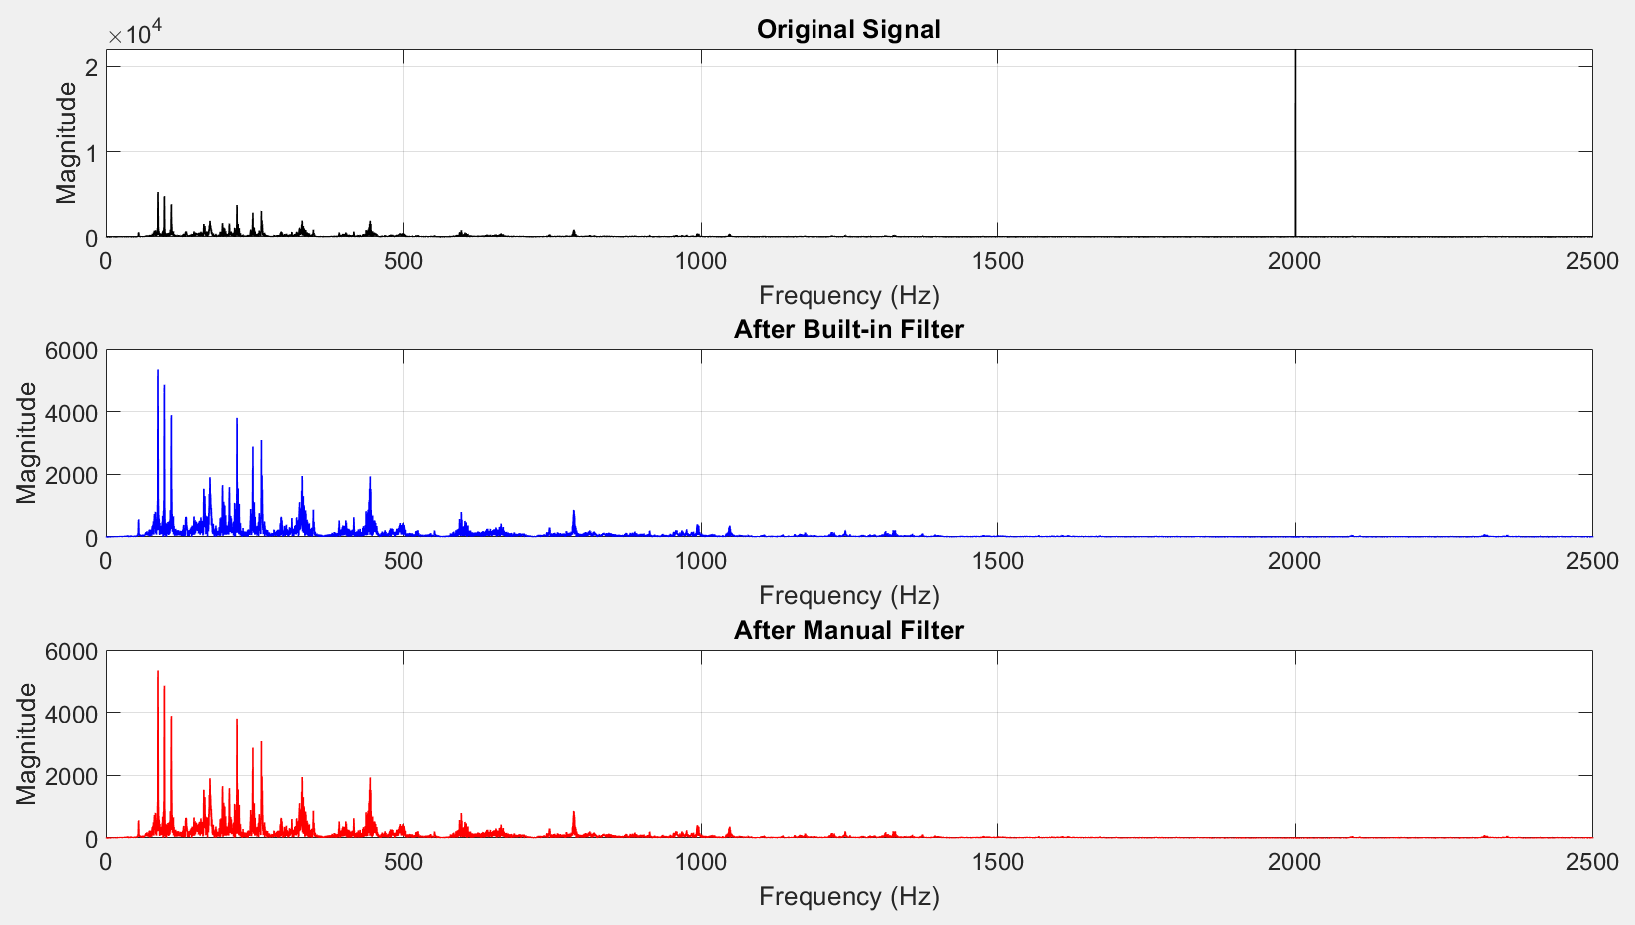
\includegraphics[width=0.9\linewidth]{before_and_after_filtering_fft.png}
    \caption{Fast Fourier Transform for Before and after filtering.}
    \label{fig:before_after_filtering}
\end{figure}


\section{Problems}
\begin{enumerate}[label=P1.\arabic*]
    \item The function $x[n]$ is defined as:    
    \begin{align*}
        x[n] = \begin{cases}
            3 & \text{for } n = 3 \\
            1 & \text{for } n = 5 \\
            -1 & \text{for } n = 7 \\
            -3 & \text{for } n > 8 \\
            0 & \text{otherwise}
        \end{cases}
    \end{align*}

    We can determine the unilateral Z-transform of $x[n]$ by using the following formula:
    \begin{align*}
        X(z) = \sum_{n=0}^{\infty} x[n]z^{-n}
    \end{align*}

    Substituting the values of $x[n]$ into the formula, we get:
    \begin{align*}
        X(z) &= 3z^{-3} + z^{-5} - z^{-7} - 3\sum_{n=9}^{\infty} z^{-n} \\
        &= 3z^{-3} + z^{-5} - z^{-7} - 3\left(\frac{z^{-9}}{1 - z^{-1}}\right) \\
    \end{align*}

    \item We can use the definition of the z-transform and then determine its region of convergence (ROC).
    \begin{enumerate}
        \item The z-transform of $x[n] = \gamma^n \cos(\pi n)u(n)$ is:
        \begin{align*}
            X(z) &= \sum_{n=0}^{\infty} \gamma^n \cos(\pi n)z^{-n} \\
            &= \sum_{n=0}^{\infty} \gamma^n(-1)^n z^{-n} \\
            &= \sum_{n=0}^{\infty} (-\gamma z^{-1})^n \\
            &= \frac{1}{1 + \gamma z^{-1}}
        \end{align*}
        The ROC is $|z| > |\gamma|$. This is because for this summation to converge, the ratio $|\gamma z^{-1}|$ must be less than 1.
        \begin{align*}
            |\gamma z^{-1}| < 1 \implies |z| > |\gamma|
        \end{align*}

        \item The z-transform of $x[n] = \left[2^{n-1} - (-2)^{n-1}\right]u(n)$ is given by:
        \begin{align*}
            X(z) &= \sum_{n=0}^{\infty} \left[2^{n-1} - (-2)^{n-1}\right]z^{-n} \\
            &= \sum_{n=0}^{\infty} 2^{n-1}z^{-n} - \sum_{n=0}^{\infty} (-2)^{n-1}z^{-n} \\
            &= \frac{1}{2}\sum_{n=0}^{\infty} \left(\frac{2}{z}\right)^n + \frac{1}{2}\sum_{n=0}^{\infty} \left(\frac{-2}{z}\right)^n \\
            &= \frac{1}{2}\left(\frac{1}{1 - \frac{2}{z}}\right) + \frac{1}{2}\left(\frac{1}{1 + \frac{2}{z}}\right) \\
            &= \frac{z}{2z - 4} + \frac{z}{2z + 4} \\
            &= \frac{z^2}{z^2 - 4}
        \end{align*}

        The radius of convergence for this is:
        \begin{align*}
            \left|\frac{2}{\left|z\right|}\right| < 1 \implies \left|z\right| > 2
        \end{align*}
    \end{enumerate}

    \item We can find the inverse z-transform of the following functions.
    \begin{enumerate}
        \item The inverse z-transform of $X(z) = \frac{(z-1)^2}{z^3}$ is:   
        \begin{align*}
            X(z) &= \frac{(z-1)^2}{z^3} \\
            &= \frac{z^2 - 2z + 1}{z^3} \\
            &= z^{-1} - 2z^{-2} + z^{-3}
        \end{align*}
        We use the common z-transform pairs to find the inverse z-transform:
        \begin{align*}
            z^{-n_0} \longleftrightarrow \delta(n-n_0)
        \end{align*}
        Therefore, the inverse z-transform of $X(z)$ is:
        \begin{align*}
            x[n] = \delta[n-1] - 2\delta[n-2] + \delta[n-3]
        \end{align*}
        
        \item The inverse z-transform of $X(z) = \frac{z-4}{z^2-5z+6}$ can be found first by doing a partial fraction decomposition:
        \begin{align*}
            X(z) &= \frac{z-4}{z^2-5z+6} = \frac{z-4}{(z-2)(z-3)} \\
            &= \frac{A}{z-2} + \frac{B}{z-3} \\
        \end{align*}

        We can then use the cover-up method to find the values of $A$ and $B$:
        \begin{align*}
            A: \text{Let z = 2} \implies A = \frac{2-4}{2-3} = 2 \\
            B: \text{Let z = 3} \implies B = \frac{3-4}{3-2} = -1
        \end{align*}
        We now have:
        \begin{align*}
            X(z) &= \frac{2}{z-2} - \frac{1}{z-3}
        \end{align*}

        We use the following transform pair:
        \begin{align*}
            \gamma^{n-1} u[n-1] \longleftrightarrow \frac{1}{z-\gamma}
        \end{align*}

        Therefore, the inverse z-transform of $X(z)$ is:
        \begin{align*}
            x[n] &= 2(2^{n-1})u[n-1] - (3^{n-1})u[n-1] \\
            &= (2^{n} - 3^{n-1})u[n-1]
        \end{align*}
    \end{enumerate}
\end{enumerate}


% --------------------------------------------------------------------------------
% END BODY
% --------------------------------------------------------------------------------

\end{document}
